\chapter{Results}\label{chp:results}

In this chapter, we present the results of different networks. Every section from \ref{sec:res} to \ref{sec:gogl} presents the results for each network. every section is divided in three subsection: one in which we discuss the results of different initialization one where we discuss the results of different optimizers and one in which the results for different classes are presented. 
\section{Resnet}\label{sec:res}
\subsection{Initialization}
For every class, we tested our network with either random initialization or with using pretrained weights. In Table \ref{tab:resinit}, we can see the best accuracy on validation and test set, the number of epochs for training for each class.  

\begin{table}
\caption{\label{tab:resinit} The results of training ResNet18 using random initialization or pretrained weights with Adamax as optimizer}
\centering
\begin{tabular}[b]{| l | l | l | l | l |}
\hline
    Initialization & Class & Validation accuracy & Test accuracy & Epochs\ \\ \hline
    \multirow{}{}{Pretrained Weights} & Dunham &  62\% & 34\% & 50 \\ 
    & Porosity & 75\% & 45\% &  50 \\
    &DRT & 75\% & 45\% &  50 \\
    &Components & 75\% & 45\% &  50 \\ \hline
     \multirow{}{}{Random} & Dunham &  62\% & 34\% & 50 \\
    & Porosity & 75\% & 45\% &  50 \\
    &DRT & 75\% & 45\% &  50 \\
    &Components & 75\% & 45\% &  50 \\ \hline
    
\end{tabular} 
\end{table}
On Figure\ref{fig:}, we plotted the accuracy, F1 score, and average training and validation loss for each class. 



\begin{figure}
\begin{subfigure}{.5\textwidth}
  \centering
  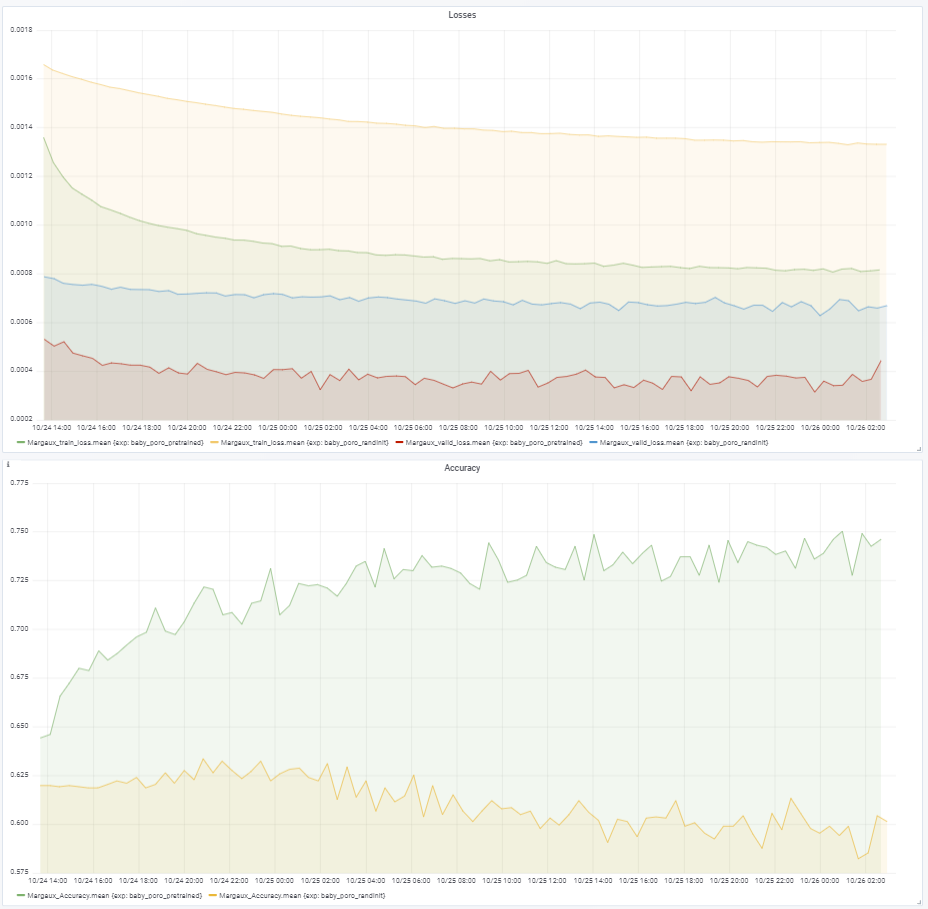
\includegraphics[width=.8\linewidth]{figures/04-Init_poro_acc.PNG}
  \caption{Resnet18 trained on the Porosity class.}
  \label{fig:resinit_poro}
\end{subfigure}%
\begin{subfigure}{.5\textwidth}
  \centering
  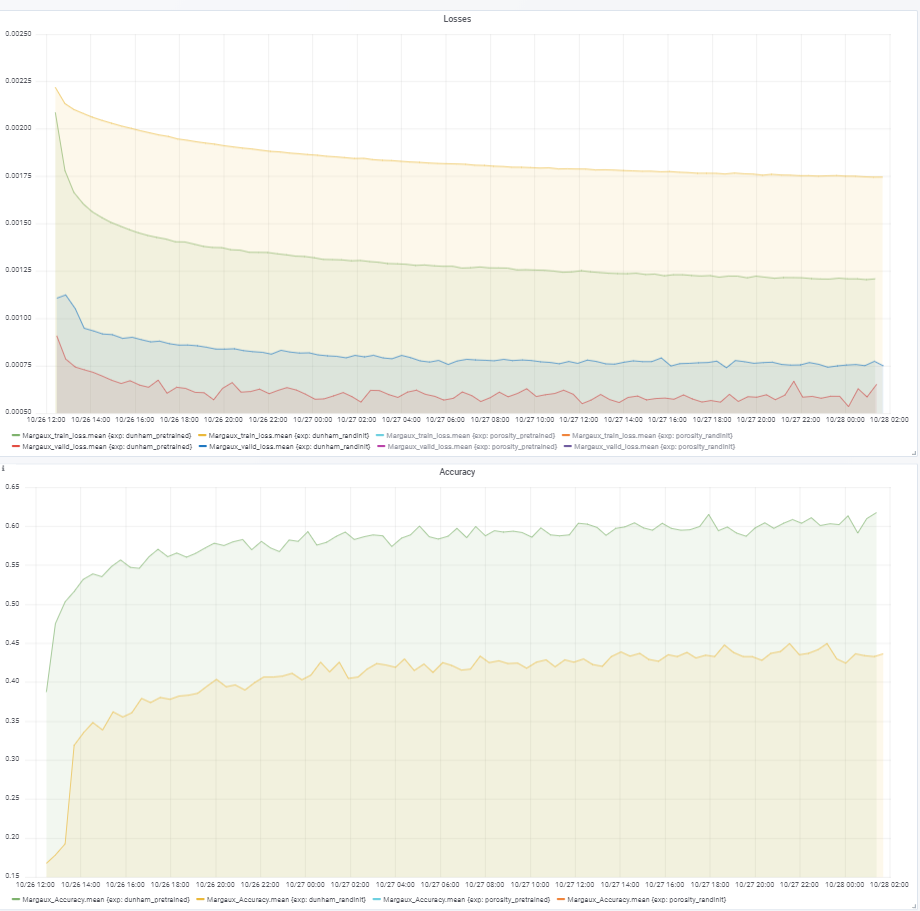
\includegraphics[width=.8\linewidth]{figures/04-Init_dunham_acc.PNG}
  \caption{Resnet18 trained on the Dunham class.}
  \label{fig:resinit_dunham}
\end{subfigure}
\begin{subfigure}{.5\textwidth}
  \centering
  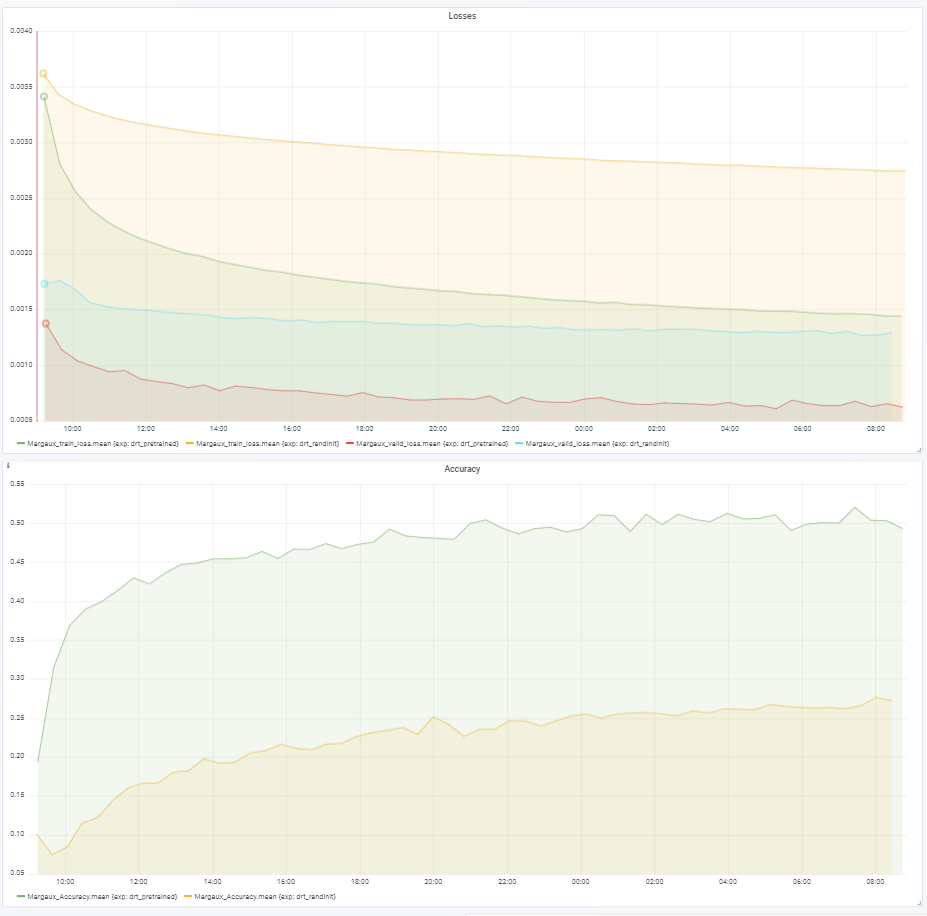
\includegraphics[width=.8\linewidth]{figures/04-Init_drt_acc.PNG}
  \caption{Resnet18 trained on the DRT class.}
  \label{fig:resinit_drt}
\end{subfigure}%
\begin{subfigure}{.5\textwidth}
  \centering
  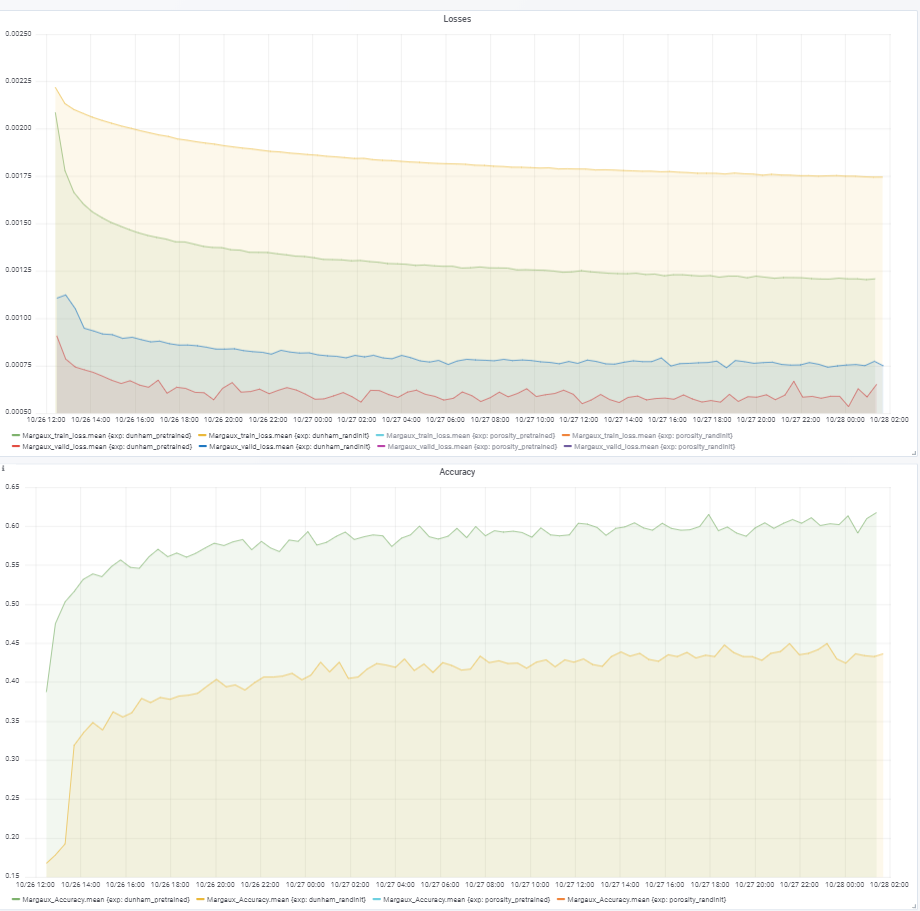
\includegraphics[width=.8\linewidth]{figures/04-Init_dunham_acc.PNG}
  \caption{Resnet18 trained on the Components class.}
  \label{fig:resinit_compo}
\end{subfigure}
\caption{The lines in green and red are for pretrained weights and yellow and blue for random initialization. The top plot is the validation accuracy and the bottom plot is training  and validation loss.}
\label{fig:fig}
\end{figure}

\subsection{Optimizer}
\subsection{Classification}
On Table\ref{tab:resbest}, we summarize the best accuracies for every class. Then on Figure
\section{AlexNet}\label{sec:aleX}
\subsection{Initialization}
\subsection{Optimizer}
\subsection{Classification}
\section{GoogleNet}\label{sec:gogl}
\subsection{Initialization}
\subsection{Optimizer}
\subsection{Classification}